\documentclass[conference]{IEEEtran}
\IEEEoverridecommandlockouts
% The preceding line is only needed to identify funding in the first footnote. If that is unneeded, please comment it out.
\usepackage{cite}
\usepackage{amsmath,amssymb,amsfonts}
\usepackage{algorithmic}
\usepackage{graphicx}
\usepackage{textcomp}
\usepackage{xcolor}
\usepackage{svg}
\usepackage{gensymb}
\usepackage{subfigure}
\DeclareMathOperator{\argmin}{\arg\!\min}
% Expectation symbol
\DeclareMathOperator{\E}{\mathbb{E}}
\def\BibTeX{{\rm B\kern-.05em{\sc i\kern-.025em b}\kern-.08em
    T\kern-.1667em\lower.7ex\hbox{E}\kern-.125emX}}
\begin{document}

\title{Learning Representative Vessel Trajectories Using Behavioral Cloning\\}

\author{\IEEEauthorblockN{1\textsuperscript{st} Anonymous Authors}
\IEEEauthorblockA{\textit{Anonymous Department} \\
\textit{Anonymous Organization} \\
Anonymous City, Anonymous Country \\
anon.email@domain.com}
}

\maketitle

\begin{abstract}
We suggest an approach to predict vessel trajectories by mimicking the underlying  policy of human captains. Decisions made by those experts are recorded by the AIS signals and can be fused with additional non-kinematic factors like weather conditions or surrounding ships to get a more accurate snapshot of the situation that led to chosen maneuvers. Here we Behavioral Cloning on a provisionally low-dimensional observation space to generate end-to-end vessel paths while incorporating time in addition to geometry. The results are promising in terms of accuracy. Extension of the method to higher-dimensional state spaces is outlooked.
\end{abstract}

\begin{IEEEkeywords}
behavioral cloning, vessel, path prediction, imitation, {reinforcement} learning
\end{IEEEkeywords}

\section{Introduction}
Including a robust model that is capable of predicting accurate future vessel paths to any maritime surveillance system is very advantageous as it improves the overall situational awareness. In this context, the ability to generate end-to-end trajectories can be utilized in a variety of different tasks e.g. detecting anomalous ship behaviour or collision avoidance.
\par
However, building such a sophisticated model is a challenging task because real-world ship maneuvering not only depends on movement indicators (current position, speed, heading) but also on a wide range of non-kinematic factors (e.g. weather conditions, current, tides and surrounding ships). In addition to the high-dimensional and semantically varying feature space, a suitable system has to also incorporate a time component and retain low computational costs intending to potentially provide near real-time predictions in short time intervals.
\par
We approach this task from the perspective of imitation learning where an artificial agent tries to extract and mimic the behaviour of human captains in order to generate similar or almost identical vessel trajectories. One major assumption is that, by learning from huge amounts of historical expert decisions under certain environmental situations, the agent acquires the skill to generalize well enough to also assemble tracks based on states it did not encounter before.

\section{Imitation Learning}

\subsection{Relationship with Reinforcement Learning}
Imitation Learning is the general approach of extracting the underlying policy given a fixed dataset of expert trajectories. Those trajectories are sampled from an environment which can be  formalized as Markov Decision Process (MDP). This framework consists of an agent which observes the current state of the environment $s_t \in \mathcal{S}$ and interacts with it in discrete timesteps by choosing an appropriate action $a_t \in \mathcal{A}$ based on a policy $\pi: \mathcal{S} \rightarrow \mathcal{A}$. The environment then provides the next state $s_{t+1}$ given the internal transition dynamics $p(s_{t+1} \mid s_t, a_t)$  and a scalar reward derived from a hand-crafted reward function $r(s_t, a_t)$ that indicates whether the proposed action was "good" or "bad".
\par
Solving such a sequential decision problem is typically achieved by applying Reinforcement Learning which uses the feedback of the environment (the reward signal) to improve the policy with an effort to maximize the discounted sum of future rewards. In fact, Reinforcement Learning has been used for the path following problem \cite{martinsen2018curved} or predicting vessel trajectories \cite{etemad2020using, zare2021continuous, s20020426}. However those approaches either do not incorporate time or take place in the very distinct field of autonomous control. 
\par
Reinforcement Learning and Imitation Learning operate within the same mathematical framework of MDPs with the exception that in the case of Imitation Learning the reward function is not required. A key difference, as designing a suitable reward function by hand that implicitly defines the desired goal can be a tedious task, especially if the reward function is non-sparse (like the \textit{Gaussian cross-track error} used in \cite{martinsen2018curved}) and the researcher tries to "guide" the agent (i.e. direct feedback at every timestep instead of a just single reward given at the very end of an episode based on the outcome).

\subsection{Behavioral Cloning}
Behavioral Cloning\cite{alvinn} reduces the task of imitating the behaviour of an expert to a supervised learning problem where a neuronal network parameterized by $\theta$ learns to map states to actions as closely as possible to the expert policy $\pi^*$. That is, it aims to minimize expected distance between actions suggested by the trained policy and the expert actions for all states encountered in the train set $(s, a^*) \sim P^*$, where $P^*(s|\pi^*)$ is the state distribution of the expert policy \cite{le2022survey}. The optimal policy is then found as:

\begin{equation}
\argmin_\theta \E_{(s,a^*) \sim P*} L(a^*, \pi_\theta(s)).
\end{equation}

\section{Experimental Setup}
\subsection{Extracting Trajectories from AIS Data}
We take historical AIS data from the coast of Bremerhaven from every first month of the quarters of the year 2020. The process of filtering and extracting single vessel trajectories is done in conjunction with the library \textit{MovingPandas}\cite{graser2019movingpandas} and can be summarized as follows:

\begin{itemize}
    \item Remove records of ships moving too slow or too fast (speed over ground is $<3$ knots or $>=30$ knots).
    \item Extract provisionally trajectories.
    \item Remove outliers based on Interquartile Range.
    \item Split trajectories that have time gaps of more than 5 minutes in consecutive AIS signals.
    \item Split trajectories by potential stops, anchoring or waiting in floodgates (ships that stay within the same area of 15 diameters for at least 3 minutes).
    \item Remove all trajectories with a length of less than 300 meters.
\end{itemize}

\begin{figure}[t]
    \centering
    \subfigure[]{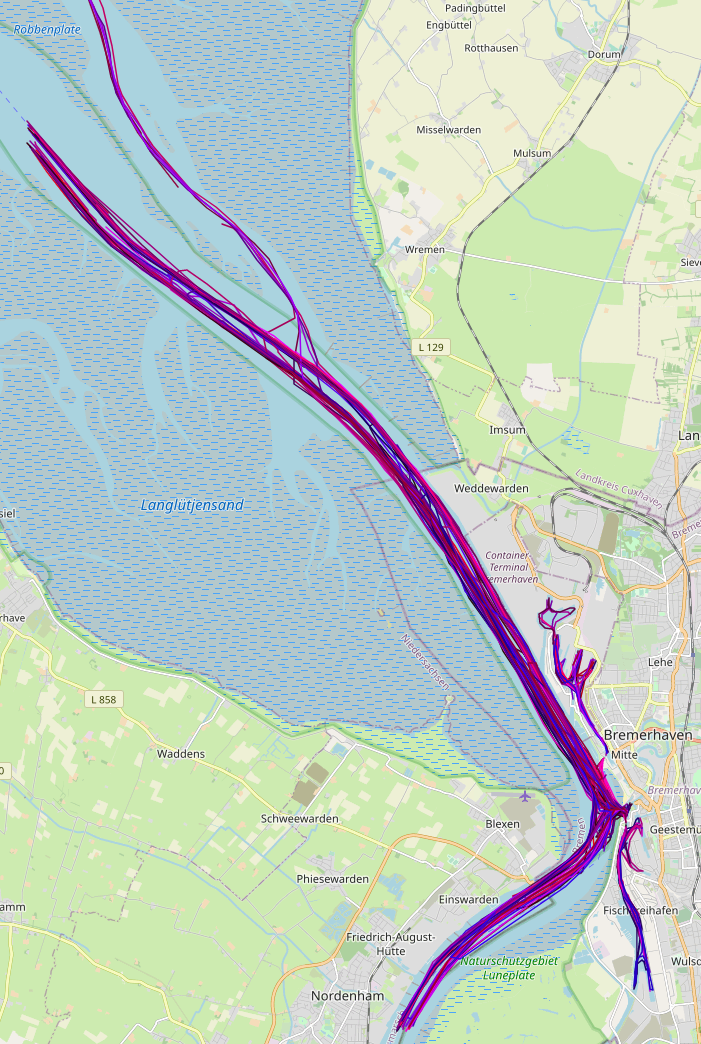
\includegraphics[width=81pt]{images/all_tracks.PNG}\label{fig:tracks}}
    \subfigure[]{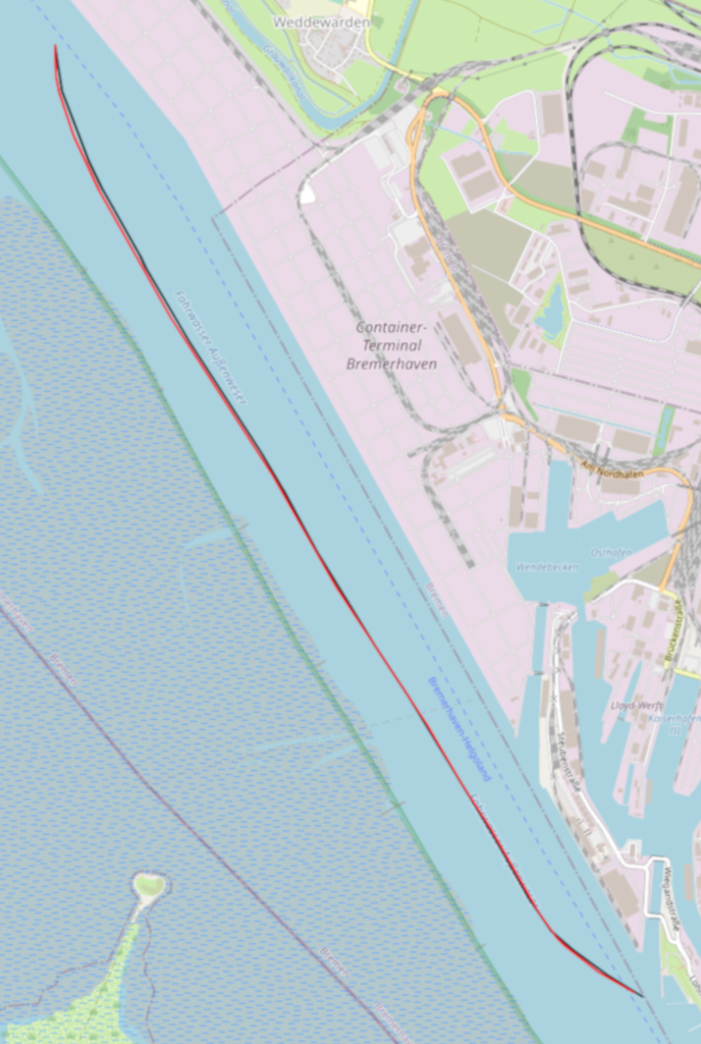
\includegraphics[width=81pt]{images/good_track.PNG}\label{fig:goodTracks}} 
    \subfigure[]{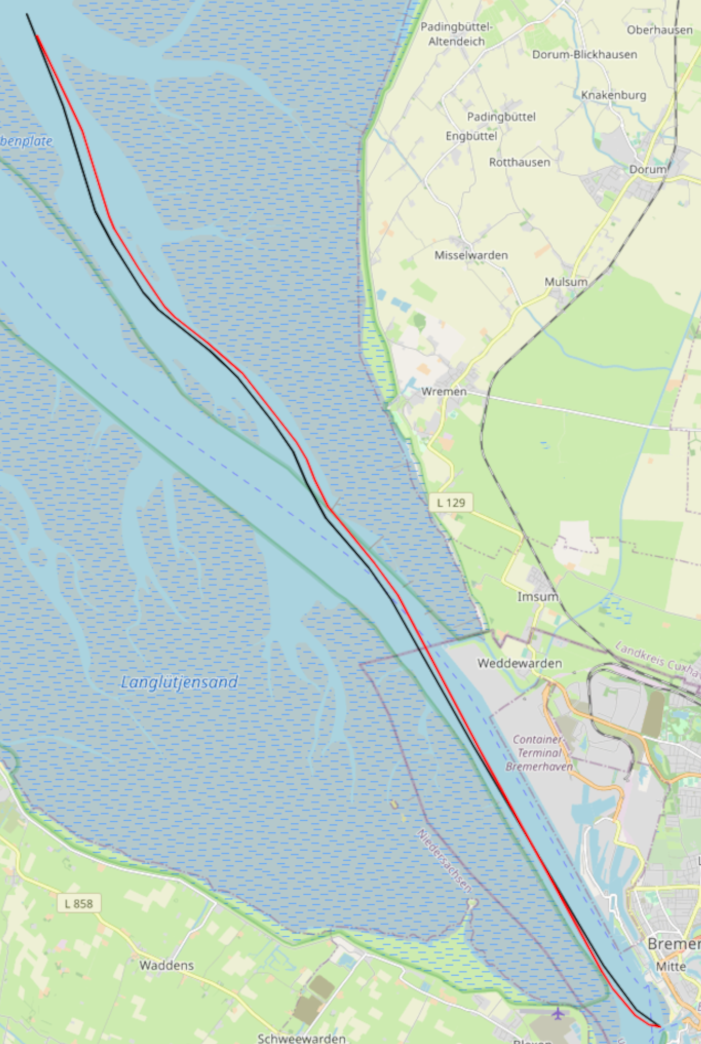
\includegraphics[width=81pt]{images/bad_track5_280.PNG}\label{fig:badTracks}}
    \caption{(a) Example of 200 extracted trajectories. Region of interest is within the bounds of longitude from $8\degree37.2'N$ to $8\degree58.8'N$ and latitude from $53\degree45.7'W$ to $53\degree72'W$.\\
    (b) and (c) display predictions in which black indicates the ground truth trajectory and red indicates the agent's prediction. (b) shows one of the most accurate predictions with an average distance of 30m. Whereas (c) is an example of what a "bad" prediction with an average distance of 280m looks like.}
    \label{fig:foobar}
\end{figure}
The resulting dataset consists of 28,000 trajectories with a subset being shown in figure \ref{fig:tracks}. In order for the system to incorporate time, the AIS records are resampled and linearly interpolated to have a fixed time interval of five seconds. Without explicitly knowing, the agent will always take actions that lead to the next state five seconds into the future.

\subsection{State Representation and Action Space}
In our first exploration, we deal with a low-dimensional feature space including only the vessel position (lon, lat), speed over ground (SoG) and course over ground (CoG). Additionally, the time component is given by the fact that consecutive states are always five seconds apart from each other. The representations of states and actions thus be defined as:
\begin{equation}
    \begin{aligned}
        s_t &:= \{lon_t, lat_t, CoG_t, SoG_t\} \\
        a_t &:= \{CoG, SoG\}
    \end{aligned}
\end{equation}

\section{Results}
To evaluate the performance of our trained policy, we use the Euclidian Distances in meters between the predicted trajectories and the true trajectories present in the test set. The results displayed in fig. \ref{fig:result} indicate that the accuracy of the prediction heavily depends on the given true trajectory. This is also empirically expressed by the high standard deviation of $\sigma=147.96m$ in relation to the overall mean distance of $\mu=178m$. In more than 3000 cases, the agent follows the given trajectory exceptionally well as displayed in fig. \ref{fig:goodTracks}. At the same time, in certain scenarios the agent does not adjust the SoG correctly which in return results in situations as illustrated in fig. \ref{fig:badTracks} where the agent is constantly trailing behind the ground truth position which in return leads to a very bad performance score. 
\begin{figure}[t]
\centering
\includesvg[width=250pt]{images/results2.svg}
\caption{Results sampled over five experiment runs with different seeds and approximately 8300 test trajectories. Trained for ten epochs with a network architecture of two fully connected hidden layers that both consist of 32 neurons.}
\label{fig:result}
\end{figure}
\section{Conclusion}
Although the results and their respective measurements to the agent's performance shown in the preceding section are fluctuating significantly, they still prove that Imitation Learning is a feasible approach to the vessel prediction task. Further investigation has to be done in order to discover what kind of trajectories or vessel types are causing bad performances. Moreover, tweaking the hyperparameters and network architecture should substantially increase the prediction accuracy.
\par
Finally, we expect to include non-kinematic features into the state representation in upcoming experiments.

\bibliographystyle{IEEEtran}
\bibliography{sources}

\end{document}
